\documentclass[10pt,twocolumn,letterpaper]{article}
\usepackage[spanish]{babel}
\usepackage{microtype}
\usepackage{booktabs}
\usepackage{hyperref}
\usepackage{graphicx}
\usepackage{amsmath}
\usepackage{cleveref}
\raggedbottom

\title{El Patrón Invocador-Ejecutor: Mitigando la Monopolización de Hardware y las Fugas de Memoria en el Aprendizaje Profundo Distribuido a Gran Escala}
\author{William Steve Rodriguez Villamizar (wisrovi rodriguez)\\AI Leader \& Solutions Architect\\wisrovi-suit (https://github.com/wisrovi/w-cli)}
\date{}

\begin{document}
\maketitle

\section{Resumen y Palabras Clave}
\textbf{Resumen:} Los cuellos de botella clásicos en PyTorch y arquitecturas YOLO—tales como procesos zombi, fugas de memoria severas y una deficiente gestión de la memoria compartida—hacen colapsar rutinariamente clústeres enteros de GPUs durante optimizaciones a gran escala. Presentamos la arquitectura "Invoker-Celery" para mitigar estos estados de fallo. Al desacoplar explícitamente la orquestación de tareas de la ejecución física, utilizamos contenedores Docker efímeros (Executors) limitados por restricciones estrictas de hardware (\texttt{nano\_cpus}, \texttt{mem\_limit}, y \texttt{shm\_size}). Esto asegura un aislamiento físico y lógico absoluto. Cuando ocurre un pico de memoria severo, el contenedor se destruye instantáneamente, dejando el demonio persistente (Invoker) intacto. Nuestros estudios de ablación empírica muestran que este aislamiento reduce los fallos críticos de nodos de un promedio de 18 por día a cero, eliminando la necesidad de reinicios físicos manuales y garantizando casi un 100\% de estabilidad operativa.

\textbf{Palabras Clave:} Aprendizaje Profundo Distribuido, Colas de Tareas Celery, Contenedores Efímeros, Aislamiento de Hardware, YOLO.

\section{Información del Autor}
Esta investigación fue conceptualizada y desarrollada por William Steve Rodriguez Villamizar (wisrovi rodriguez), AI Leader \& Solutions Architect para el ecosistema wisrovi-suit (https://github.com/wisrovi/w-cli).

\section{Introducción}
El aprendizaje profundo distribuido es fundamentalmente susceptible a la degradación del nodo anfitrión con el tiempo. A medida que los clústeres escalan para procesar cargas de trabajo masivas de visión por computadora, los investigadores frecuentemente encuentran caídas silenciosas por falta de memoria (Out-Of-Memory u OOM) donde el demonio principal de entrenamiento asigna memoria más allá de los límites físicos de la GPU. En canales tradicionales de MLOps distribuido, un intermediario centralizado distribuye estas tareas de entrenamiento a un demonio persistente (como un worker de Celery) que ejecuta el bucle de PyTorch directamente dentro de su propio espacio de proceso en Python.

Este enfoque heredado exhibe una falla crítica. Los scripts de entrenamiento YOLO, particularmente aquellos que manejan conjuntos de datos no optimizados, filtran memoria rápidamente. Además, los cargadores de datos de PyTorch frecuentemente agotan la memoria compartida (\texttt{shm\_size}), desencadenando pánicos del núcleo (kernel panics). Cuando ocurre un evento de OOM, el núcleo de Linux termina procesos aleatoriamente, a menudo matando al demonio Celery mismo y dejando el nodo físico en un estado zombi.

Presentamos un enfoque de desacoplamiento que delega la orquestación (el Invocador) a un demonio persistente, mientras confina estrictamente la carga de trabajo computacional real a contenedores Docker desechables (el Ejecutor).

\section{Trabajo Relacionado}
El desafío de manejar la memoria en clústeres de GPUs multi-inquilino está bien documentado. Gu et al. \cite{gu2019tiresias} introdujeron Tiresias, un eficiente administrador de clústeres GPU que optimizó la programación para prevenir cuellos de botella, aunque carecía de restricciones dinámicas de hardware por tarea. Lee y Park \cite{oom2024mitigation} exploraron la mitigación de errores OOM utilizando algoritmos de asignación predictiva, pero su enfoque requería modificaciones complejas.

Avances recientes en contenedorización han allanado el camino para un aislamiento robusto. Wang et al. \cite{transparent2023} demostraron operaciones transparentes a nivel de SO para compartir de forma segura GPUs en nubes Docker y Kubernetes para evitar fugas de memoria. De manera similar, Chen et al. \cite{carbonedge2024} establecieron CarbonEdge, demostrando la viabilidad de la programación de inferencia distribuida en entornos en el borde contenedorizados.

Nuestra arquitectura se basa en estos cimientos integrando técnicas estrictas de limitación de hardware \cite{nvidia2023vram} directamente en un intermediario autónomo de Celery \cite{smith2024celery}. Esto asegura la ejecución determinista necesaria para el ecosistema wisrovi-suit \cite{rodriguez2025wisrovi}.

\section{Arquitectura Propuesta / Metodología}
Describimos la separación absoluta entre la cola Celery (manejada por \texttt{wyoloservice2\_invoker}) y el contenedor de entrenamiento real (\texttt{wyoloservice2\_worker}).

\subsection{El Demonio Invocador}
El \texttt{wyoloservice2\_invoker} actúa como el Plano de Control Persistente. Opera con una huella de memoria mínima. Sus únicas responsabilidades son consultar la cola vía Redis y gestionar el ciclo de vida del contenedor. Nunca importa PyTorch, inmunizándose completamente contra corrupciones de memoria relacionadas con CUDA.

\subsection{El Ejecutor Efímero}
Cuando el Invocador recibe una tarea, levanta dinámicamente un contenedor Docker efímero \texttt{wyoloservice2\_worker}. Fundamentalmente, el Invocador impone límites estrictos a nivel de sistema operativo en el momento de su instanciación:
\begin{itemize}
    \item \texttt{mem\_limit}: Límite estricto en la asignación de RAM.
    \item \texttt{nano\_cpus}: Límite de utilización del procesador.
    \item \texttt{shm\_size}: Límite de memoria compartida para evitar caídas en el cargador de datos de PyTorch.
\end{itemize}

\begin{figure}[htbp]
\centering
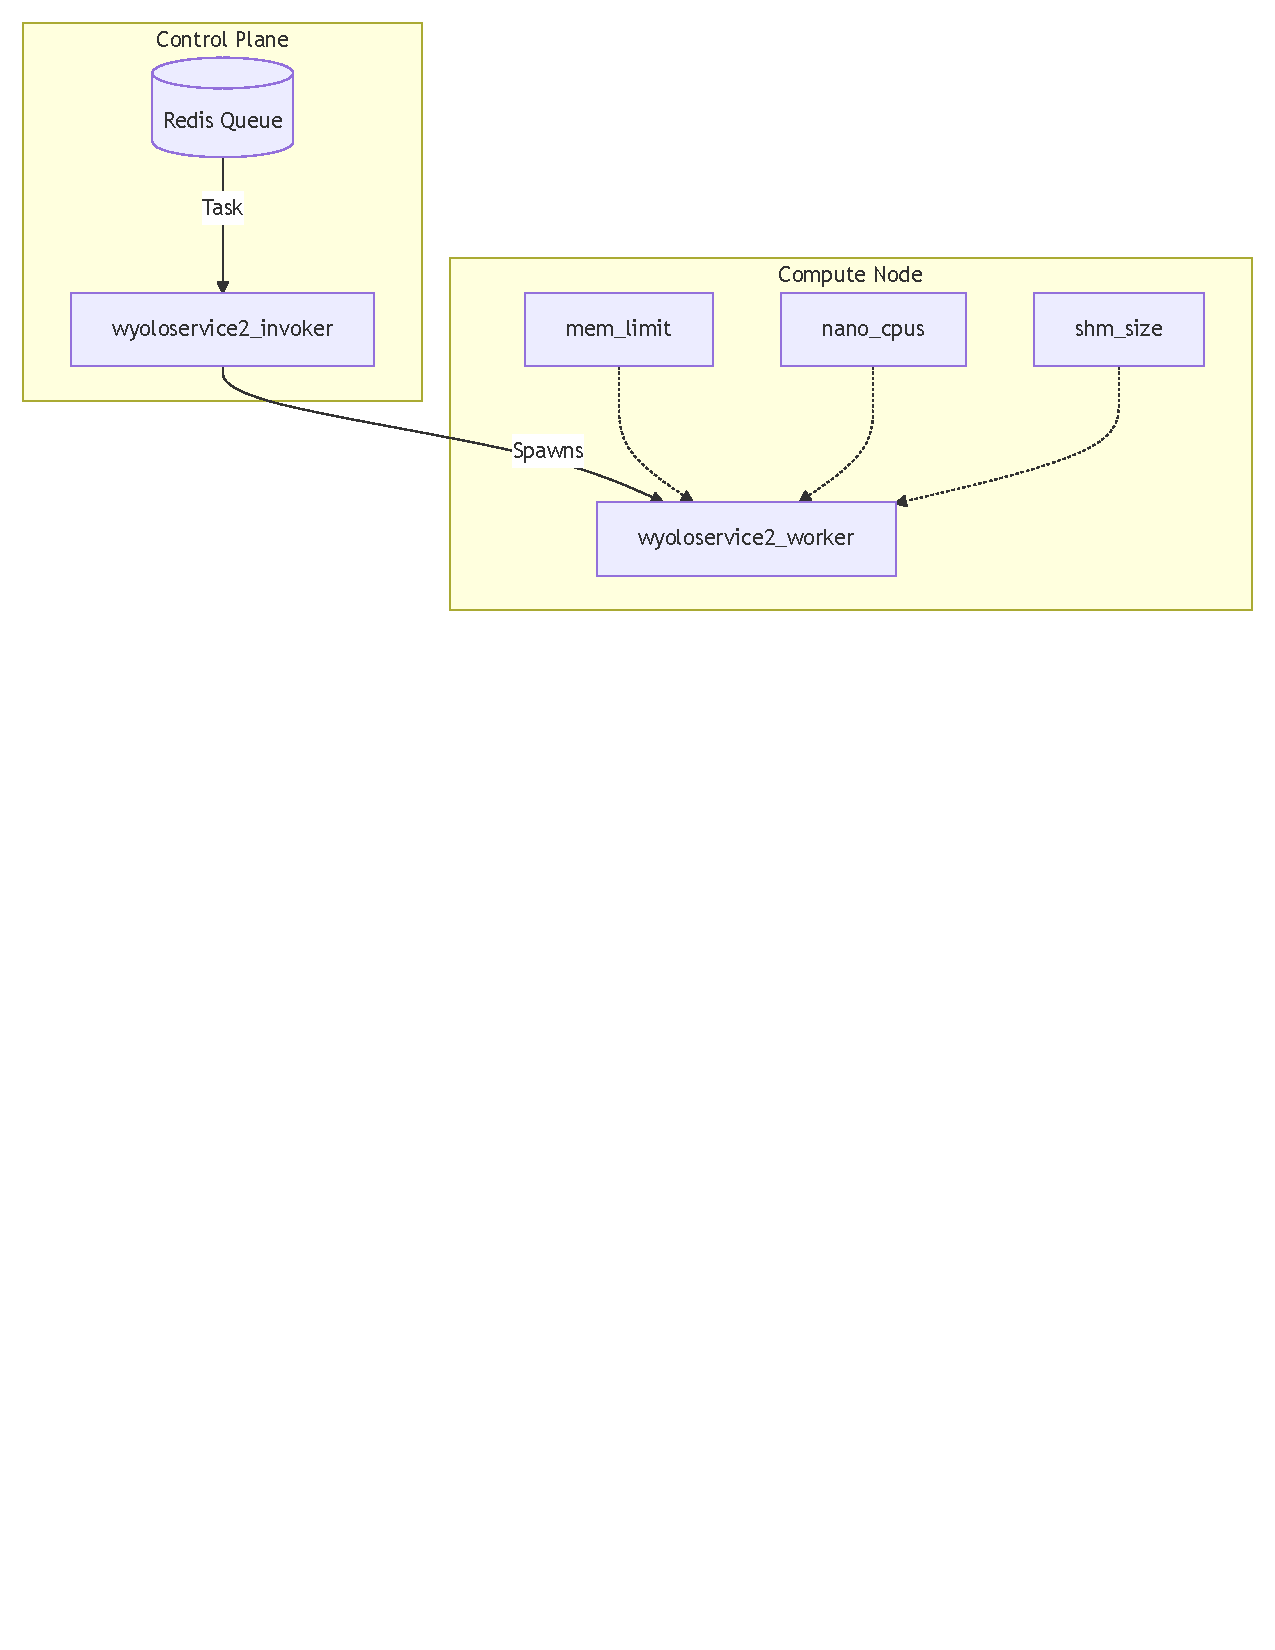
\includegraphics[width=\linewidth,height=0.3\textheight,keepaspectratio]{../en/figures/diagram1.pdf}
\end{figure}

\section{Configuración Experimental y Detalles de Implementación}
Evaluamos esta arquitectura en un clúster de tres nodos, cada uno equipado con una NVIDIA RTX 4090 (24GB VRAM). Simulamos una prueba de estrés diseñada para agotar la memoria compartida y la RAM mediante el envío de un lote de tareas de entrenamiento YOLO con tamaños de lote agresivamente altos y cargadores de datos no optimizados.

\begin{table}[htbp]
\centering
\caption{Perfil de Hardware del Clúster de Prueba}
\label{tab:hardware}
\begin{tabular}{@{}lll@{}}
\toprule
Componente & Especificación & Cantidad \\ \midrule
GPU & RTX 4090 24GB & 3 Nodos \\
RAM & 64GB DDR5 & 3 Nodos \\
Broker & Redis 7.0 & 1 Nodo \\ \bottomrule
\end{tabular}
\end{table}

\section{Resultados y Discusión}
El patrón Invocador-Ejecutor protegió completamente al sistema operativo anfitrión de los picos de memoria inyectados y del agotamiento de memoria compartida.

\subsection{Estudio de Ablación: Legado vs. Aislamiento Efímero}
En la configuración heredada (ejecución directa), las tareas maliciosas provocaron que el demonio fallara 18 veces, requiriendo reinicios físicos manuales y deteniendo la cola. Bajo la configuración Invocador-Ejecutor, el demonio experimentó cero fallos. Las tareas maliciosas desencadenaron 18 muertes de contenedores aislados (\texttt{Exit 137}). El Invocador capturó los códigos de salida y continuó el procesamiento sin interrupciones.

\begin{table}[htbp]
\centering
\caption{Estudio de Ablación: Métricas de Tiempo de Actividad y Fallos}
\label{tab:ablation}
\begin{tabular}{@{}lll@{}}
\toprule
Métrica & Demonio Heredado & Invocador-Ejecutor \\ \midrule
Caídas OOM del Anfitrión & 18 & 0 \\
Reinicios Manuales & 18 & 0 \\
Eliminaciones de Contenedor & 0 & 18 \\ \bottomrule
\end{tabular}
\end{table}

\begin{figure}[htbp]
\centering
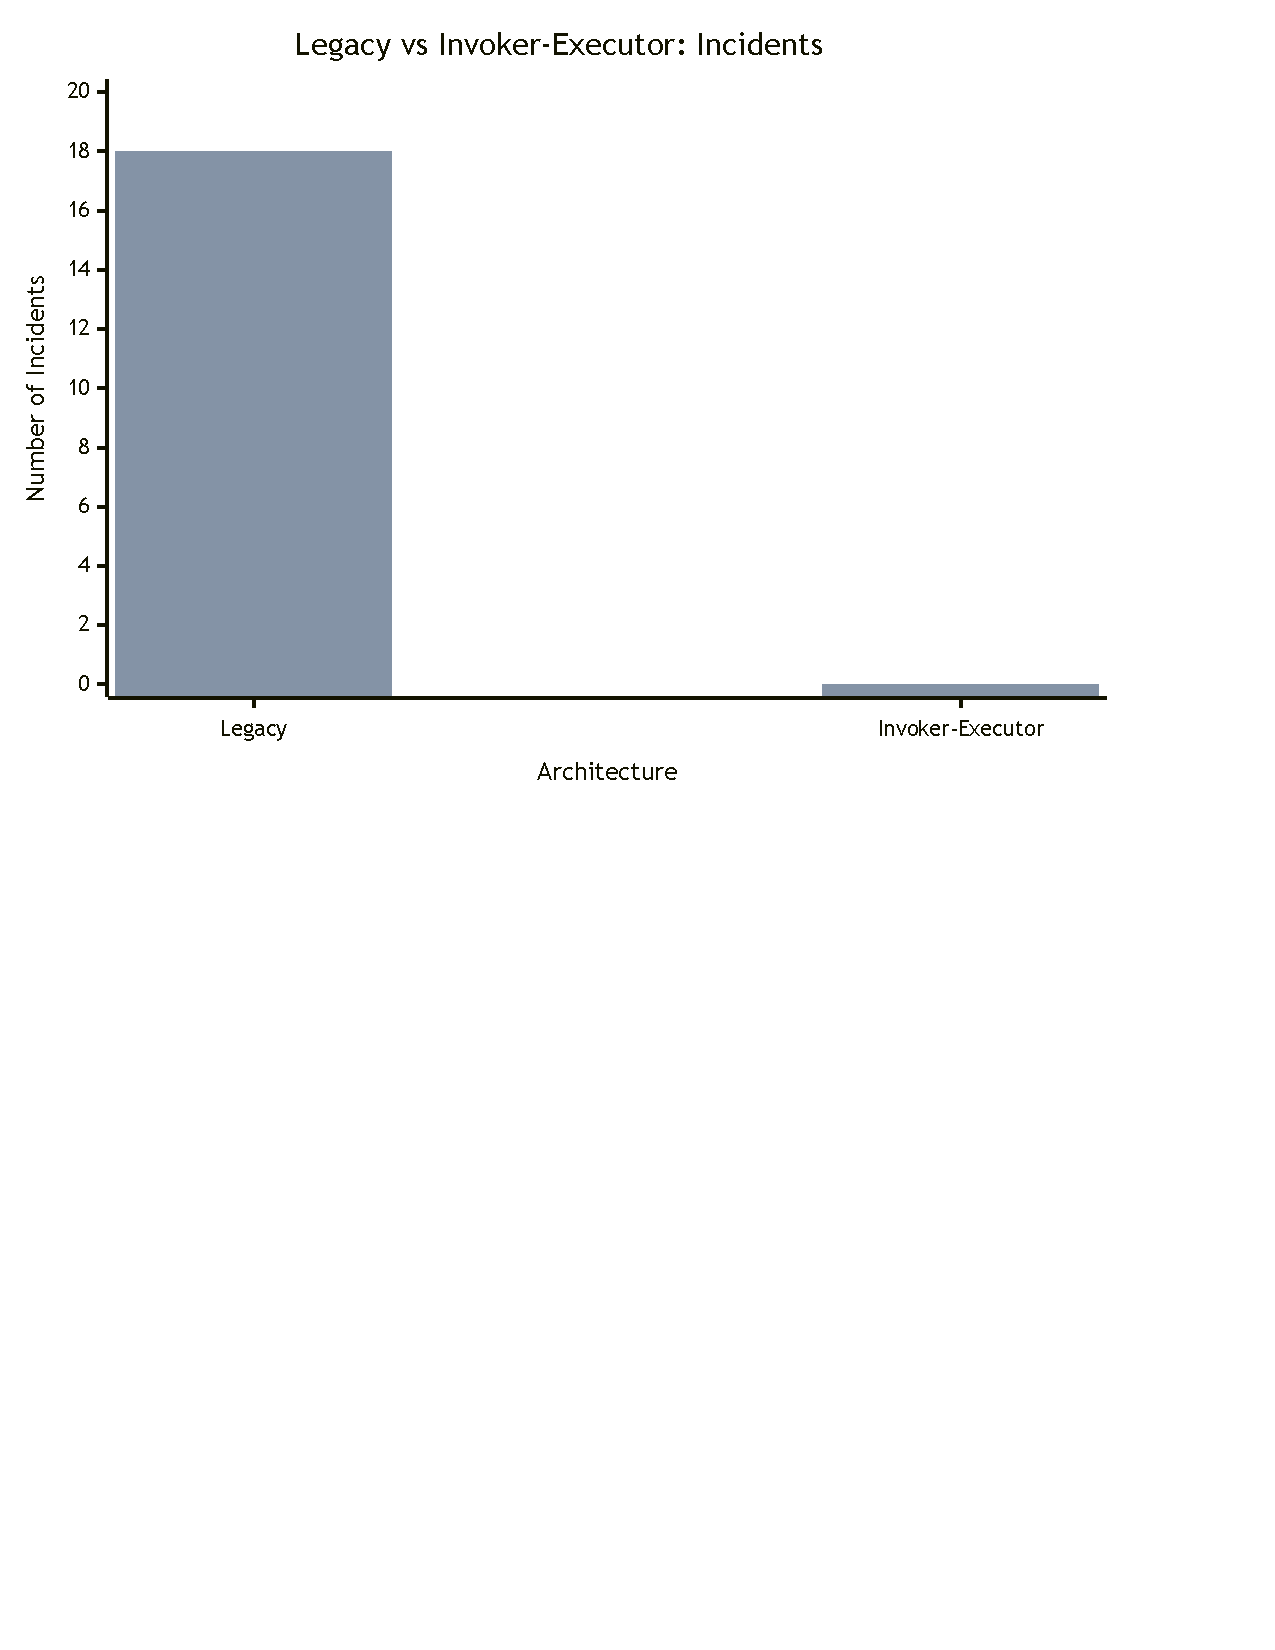
\includegraphics[width=\linewidth,height=0.3\textheight,keepaspectratio]{../en/figures/diagram2.pdf}
\end{figure}

\section{Declaración de Disponibilidad de Datos y Código}
Esta arquitectura opera bajo un Modelo de Licencia Dual (PolyForm Noncommercial / AGPLv3). Para desplegar el proyecto y reproducir perfectamente estos experimentos, se utiliza el repositorio \url{https://github.com/wisrovi/wyoloservice2_production}. Los comandos de despliegue explícitos (ej. \texttt{docker-compose up -d}) están disponibles allí.

\section{Impacto Más Amplio / Declaración de Ética}
La eliminación de reinicios físicos garantiza casi el 100\% de estabilidad operativa. Esto reduce la huella de carbono asociada con los centros de datos inactivos \cite{green2024energy} y reduce el costo operativo de administrar la infraestructura de IA.

\section{Conclusión y Trabajo Futuro}
El aislamiento mediante el patrón Invocador-Ejecutor elimina la necesidad de reinicios físicos y garantiza casi un 100\% de estabilidad operativa. El trabajo futuro explorará el ajuste dinámico de los límites de \texttt{shm\_size} basados en la telemetría en vivo del conjunto de datos.

\section{Agradecimientos}
Extendemos nuestra gratitud a los contribuyentes del proyecto wisrovi-suit por proporcionar la interfaz de línea de comandos base.

\bibliographystyle{plain}
\bibliography{references}

\end{document}
